\documentclass[a4paper]{article}

\usepackage{color}
\usepackage{url}
\usepackage[T2A]{fontenc} 
\usepackage[utf8]{inputenc} 
\usepackage{graphicx}

\usepackage[english,serbian]{babel}

\usepackage[unicode]{hyperref}
\usepackage{color}
\hypersetup{colorlinks,citecolor=green,filecolor=green,linkcolor=blue,urlcolor=blue}

\begin{document}

	\title{Bežični prenos električne energije\\ \small{Seminarski rad u okviru kursa\\Tehničko i naučno pisanje\\ Matematički fakultet}}
	
	\author{Dobrivoje Vujovic \\mi22051@alas.matf.bg.ac.rs 
			\and Mila Gligoric \\mi22082@alas.matf.bg.ac.rs
			\and Milan Petrovic \\ adresa
			\and Boris Peric\\ adresa}

	\date{15. Novembar. 2022.}
	\maketitle

\tableofcontents
\newpage

\section{Primene}
\label{sec:Primene}
Bežični prenos električne energije, ako pravilno implementiran, ima mogućnost da unapredi veliki broj industrija. Najveća potražnja je trenutno u sektoru potrošačke elektronike, gde jedna od prvih inovacija koje možemo da očekujemo jeste stanica za punjenje na distanci od 1-5 metara. \cite{a} Ideja je da u svakom domaćinstvu postoji par predajnika za punjenje (u zavisnosti od veličine prostora) koji bi punili svu kompatibilnu elektroniku i time potpuno uklonili potrebu za standardnim žičanim punjačima. Ovo rešenje je i dalje nemoguće, delom zbog nedovoljnog razvića tehnologije, ali i zbog skepticizma prosečnog potrošača o sigurnosti rešenja tog tipa. 
\\[10pt]
Kako je magnetna rezonanca u oblasti bežičnog prenosa energije proteklih decenija zadobila na popularnosti, isti principi magnetne teorije koji se koriste za tehnološki napredak elektronike mogu se primeniti i na medicinski sektor. \cite{b} BPE sistemi (eng. WPT systems) su na putu da preobraze proizvodnju medicinskih uređaja namenjenih za upotrebu unutar tela, specifično onih koji koriste baterije i električna kola. Pejsmejkeri (eng. pacemaker) su uređaji koji regulišu rad srca, a od kojih na globalnom nivou zavise životi oko 5 miliona ljudi. Vek trajanja baterije pejsmejkera (od 5-7 godina) \cite{c} pacijenta može dovesti u ozbiljan zdravstveni rizik, zbog čega naučnici rade na kreiranju uređaja koji se pune eksterno. 
\\[10pt]
Bežični prenos energije je na putu da unapredi i automobilsku industriju. Kako se svake godine proizvodi sve više električnih vozila, traže se i inovativni načini za njihovo punjenje. Trenutno se radi na stanicama gde automobili mogu parkirani da se pune bežično. U planu za budućnost je izrada tehnologije pomoću koje će automobili moći da se napune čak i dok su u pokretu, a punjaći će biti raspoređeni po putevima tako da će vozila moći da rade bez stajanja. Kao rezultat ove promene, mnogo više ljudi bi biralo električna vozila. 
\\[10pt]
Još neke sfere u kojima koje će se bežični prenos energije koristiti:
\begin{itemize}
 \item gradjevina: uklanjanje žica iz domova
 \item odbrambeni sektor: smanjenje težine baterija na bojnom polju
 \item biomedicina: izrada protetskih uredjaja
 \item solarne ploče itd.
\end{itemize}
\section{Održivost}
\label{sec:Održivost}

Standardne primene bežičnog prenosa energije nemaju dokazan štetan uticaj na životnu sredinu. U velikoj razmeri predviđa se da će BPE proizvoditi samo 20g ugljen-dioskida, jednog od glavnih uzroka globalnog zagrevanja, po kilovatsatu. \cite{a} Obračun za nuklearnu energiju je otprilike isti, dok ga nafta emitira čak i 40x više. *„Leed“ sertifikovani profesionalci smatraju da je tehnologija bezicnog prenosa energije sastavni deo pokreta održivosti i ’zelene’ gradnje \cite{d}, posebno kako maloprodajna cena elektriciteta nastavlja da raste. Bežicna energija pruza mogucnost smanjenja potrebe za novim ožičenjem kuća i preduzeća, kao i eliminisanja potencijalno rastuće potražnje za baterijama u budućnosti (posledica povećanja energetskih potreba IoT i 5G mreže).     


\section{Svetski bežicni sistem}
\label{sec:svetskisistem}
Svetski bežicni sistem je bio projekat koji je dizajnirao Nikola Tesla na osnovu svojih teorija o korišćenju Zemlje I njene atmosfere kao električnih provodnika. Bitnost ovog projekta ogleda se u činjenici da je njime Tesla pokazao da je moguce prenositi energiju na daljinu, bez korišćenja drugih provodnika, osim vazduha. On je tvrdio da će ovaj sistem omogućiti “Prenos električne energije bez žica” na globalnom nivou, kao I bežicnu komunikaciju I emitovanje radio signala. Projekat je napusten 1906. godine zbog nedostatka sredstava I nikada posle toga nije završen.

\begin{figure}[h!]
\begin{center}
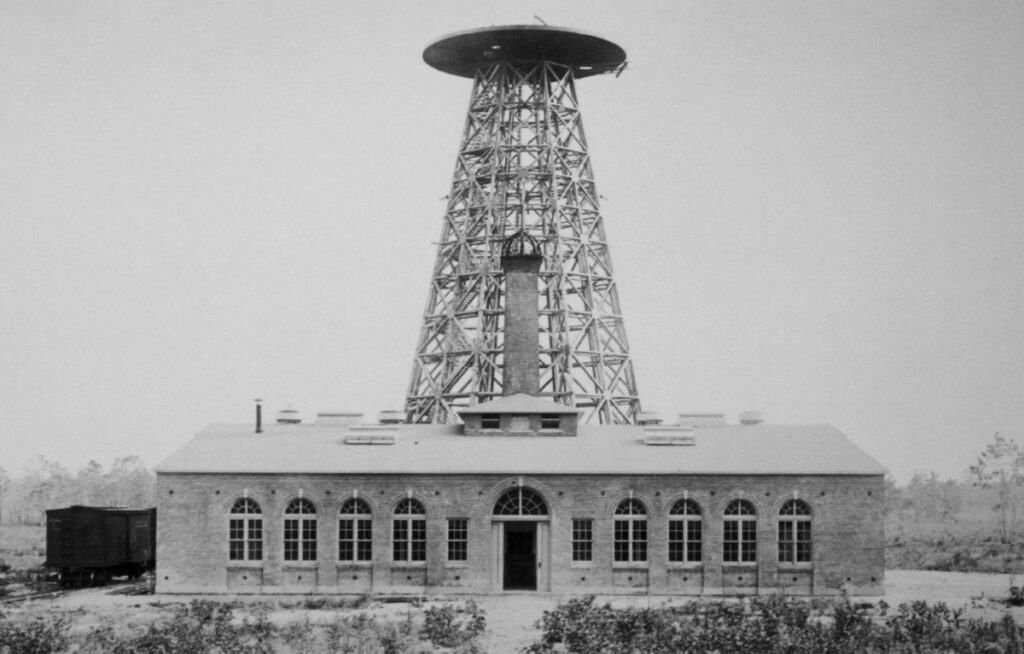
\includegraphics[scale=0.25]{toranj.jpg}
\end{center}
\caption{Teslin Toranj}
\label{fig:toranj}
\end{figure}

\subsection{Istorija}
\label{subsec:istorija}
Kada se Tesla vratio iz Kolorado Springsa u Njujork, napisao je senzacionalan članak za Century Magazine\cite{teslinClanak}. U ovoj detaljnoj, futurističkoj viziji on je opisao sredstvo za prikupljanje sunčeve energije pomoću antene. On je sugerisao da bi bilo moguce kontrolisati vremenske prilike električnom energijom. Predvideo je mašine koje će rat učiniti nemogućim. I predložio je globalni sistem bežične komunikacije. Većini ljudi ideje su bile gotovo nerazumljive, ali Tesla je bio čovek koji se nije mogao potceniti.

Ovaj članak privukao je pažnju jednog od najmoćnijih ljudi toga vremena, J.P Morgan-a. Budući da su se lično poznavali, Tesla je Morganu izložio svoju ideju, koja se tada graničila sa naučnom fantastikom. “Kada se bežična mreža u potpunosti primeni, Zemlja će se pretvoriti u ogroman mozak, sposoban da reaguje u svakom svome delu”\cite{intervju1926}, tvrdio je Tesla.

Morgan je Tesli ponudio 150 000 dolara, da napravi prenosni toranj I elektranu. Iako je Tesli trebalo mnogo više novca za projekat, prihvatio je ponudu I odmah krenuo sa radovima.


Kao mesto za svoj projekat Tesla je izabrao zemljište Vardenklif(engl. Wardenclyffe) na liticama Long Island-a. Projekat je bio u izgradnji sve do 1901. godine, a konstrukcija je uključivala toranj koji se uzdizao 57m u visinu I koji je na svom vrhu nosio čeličnu kuglu tešku 55 tona. Ispod tornja, 35 metara duboko, nalazilo se udubljenje, nalik na bunar, a par metara dublje nalazilo je se šesnaest gvozdenih cevi učvršćenih u zemlju.

Kako je izgradnja tornja odmicala, postalo je jasno da početna investicija neće biti dovoljna, ali Morgan nije reagovao. Zatim je krajem 1901. objavljena vest da je Markoni(ital. Guglielmo Marconi) signalizirao slovo “S” preko Atlantika od Kornvola u Engleskoj do Njufaundlenda, što je dalje poljuljalo Markonija u odluci da nastavi da finansira Teslin projekat.

Tesla je molio Morgana za dodatnu finansijsku podršku, ali je investitor odlučno odbio; berza je doživela krah, a cene materijala su se udvostručile. Visoke cene u kombinaciji sa neuspelim pokušajem pronalaska investitora, na kraju su dovele do propasti projekta.

\subsection{Princip Rada}
\label{subsec:principrada}
Teslina ideja za Vardenklifski toranj rodila se početkom 1890-ih godina. Glavni cilj njegovog istraživanja bio je da razvije novi sistem bežičnog prenosa energije. Odbacio je ideju o korišćenju novootkrivenih Hercovih radio Talasa, koje je 1888. otkrio nemački fizičar Hajnrih Rudolf Herc. Tesla je sumnjao u njihovo postojanje, pošto mu je osnovna fizika, kao I većini drugih naučnika iz tog perioda, govorila da će talasi  putovati pravolinijski, što znači da će putovati pravo u svemir, postajući izgubljeni.\cite{izgubljeniTalasi}

Tokom prethodnih eksperimenata izvedenih u Kolorado Springsu 1899. godine, Tesla je razvio sopstvene ideje o tome kako će funkcionisati svetski bežični sistem. Iz ovih eksperimenata izneo je teoriju da bi ako bi pustio električnu struju u Zemlju na određenoj frekvenciji, mogao da iskoristi ono za sta je verovao da je Zemljin sopstveni električni potencijal, I da izazove da struja rezonuje na frekvenciji koja bi se pojačavala po principu stojecih talasa\cite{stojeciTalasi}. Energiji ovih talasa moglo bi se pristupiti bilo gde na Zemlji za pokretanje raznih uređaja. Ovakav sistem zasnivao je se više na idejama o električnoj provodljivosti iz 19. veka umesto o modernijim teorijama o elektromagnetnim talasima.
	
Februara 1901. u Collier-ovom članku pod nazivom “Razgovor sa planetama Tesla je opisao svoj bežični sistem na sledeći način:
“Koristi Zemlju kao medijum za sprovođenje struje, oslobađajući se žica I svih drugih veštačkih provodnika ...mašina koja, da objasnim svoj rad jednostavnim jezikom, u svom delovanju podseća na pumpu, crpeći struju Iz Zemlje I vraćajući je nazad u ogromnoj brzini, stvarajući tako talasanje ili potrerse koji bi, šireći se Zemljom kao kroz žicu, mogli biti otkriveni na velikoj udaljenosti pažljivo podešenim prijemnim krugovima. Na ovaj način mogao sam da prenesem na daljinu, ne samo slabe signale, već i značajne količine energije, a kasnija otkrića koje sam imao, uverila su me da ću na kraju uspeti da prenosim energiju bežično u industrijske svrhe, uz niske cene I na bilo kojoj udaljenosti.

Iako je Tesla demonstrirao bežični prenos energije osvetljavajući sijalice postavljene ispred zgrade u kojoj je postavio svoj eksperimentalni kalem,\cite{teslinClanak} nije naučno dokazao svoje teorije. Verovao je da je postigao rezonaciju Zemlje koja bi, prema njegovoj teoriji, delovala na bilo kojoj udaljenosti.\cite{teorija}

\bibliographystyle{plain}
\bibliography{seminarski.bib}

\end{document}
